\section{Caso 4. Inferencia a través de la reutilización de ontologías. }
\label{section:caso4}

En este caso se pretende mostrar la capacidad de reutilización e inferencia para la integración de datos. Utilizamos la fuente de Procesos Licitatorios de la DNCP y la fuente de Procesos Licitatorios de Zaragoza\footnote{http://www.zaragoza.es/ciudad/risp/sparql.htm}, donde ambos reutilizan la ontología de Public Contract dentro de sus respectivas ontologías. 

La ontología OCDSPY no está anotada directamente con la clase \textit{pc:Tender} pero sí están anotados con \textit{ocds:Tender} la cual, que está definida como una subclase de \textit{pc:Tender} (como se muestra en el Cuadro \ref{lst:caso4-1}). En este caso, La Ontología de Zaragoza utiliza directamente la propiedad \textit{pc:Tender}.

\noindent\begin{minipage}[c]{\textwidth}
\begin{lstlisting}[captionpos=b, caption=Extensión de la ontología reutilizando PC, label={lst:caso4-1},  numbers=left,  numberstyle=\tiny\color{mygray},frame=single]
###  http://purl.org/onto-ocds/ocds#Tender
:Tender rdf:type owl:Class ;
        rdfs:subClassOf pc:Tender ;
        rdfs:comment "Data regarding tender process - publicly inviting prospective contractors to submit bids for evaluation and selecting a winner or winners"@en ;
        rdfs:label "Tender"@en .
 \end{lstlisting}
\end{minipage}

\subsection{Mejora: Motor de Inferencia}
Para obtener las convocatorias de la DNCP es necesario que el Punto SPARQL utilice el motor de inferencia ya que los datos no están directamente anotados con la misma clase. En el sección \ref{section:puntosparql} se vio cómo se creó y habilitó la capacidad de inferencia al Punto SPARQL\hfill \break

La consulta realizada en el Cuadro \ref{lst:caso4-2} consiste en listar los primeros 6 contratos encontrados (3 de Paraguay y 3 de Zaragoza)”.\hfill \break
 
\noindent\begin{minipage}[c]{\textwidth}
 \begin{lstlisting}[captionpos=b, caption=Consulta a dos fuentes de datos utilizando el mismo concepto, label={lst:caso4-2},  numbers=left,  numberstyle=\tiny\color{mygray},frame=single]
SELECT ?tender
WHERE {
    #Paraguay
    { 
        SELECT * 
        WHERE {
            ?tender ?b pc:Tender 
        } 
        LIMIT 3 
    }
    UNION 
    #Zaragoza
    { 
        SERVICE <http://datos.zaragoza.es/sparql> {
            SELECT * 
            WHERE {
                ?tender ?b pc:Tender 
            } 
            LIMIT 3
        }
    }
}
 \end{lstlisting}
\end{minipage}
 Los resultados obtenidos se muestran en la Figura \ref{img:caso4Resultado}. Allí se muestra el identificador de cada convocatoria. Con esta consulta, podemos estar seguros de que todos los recursos de la lista corresponden a convocatorias, aunque las convocatorias no son del mismo publicador de datos.



\begin{figure}[ht!]
    \centering
    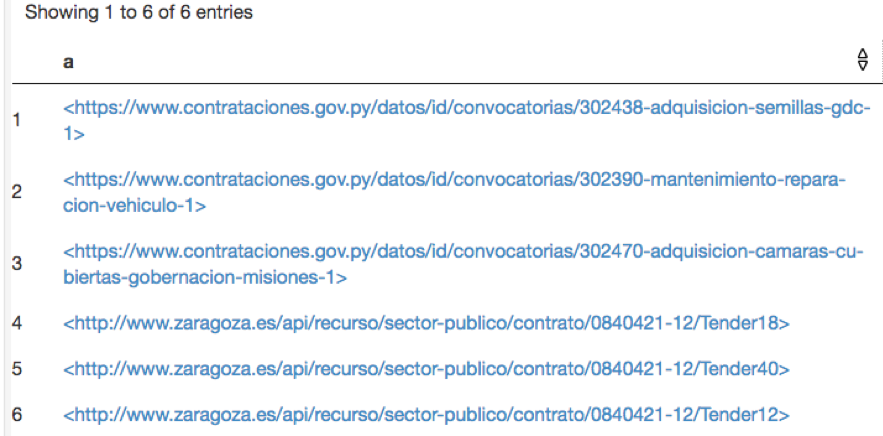
\includegraphics[width=80mm]{figuras/caso4Resultado.png}
    \caption{Despliegue de resultado de la consulta del caso 4}
    \label{img:caso4Resultado}
 \end{figure}

 En la Figura \ref{img:Diagramas-Caso 4} se observa que ambas fuentes de datos reutilizan la ontología de Public Contract, en este caso la propiedad “Tender”. Gracias a esto es posible relacionar los datos en una consulta al Punto SPARQL logrando así la interoperabilidad semántica, dando seguridad de que ambas fuentes de datos se refieren al mismo concepto.

 \begin{figure}[ht!]
    \centering
    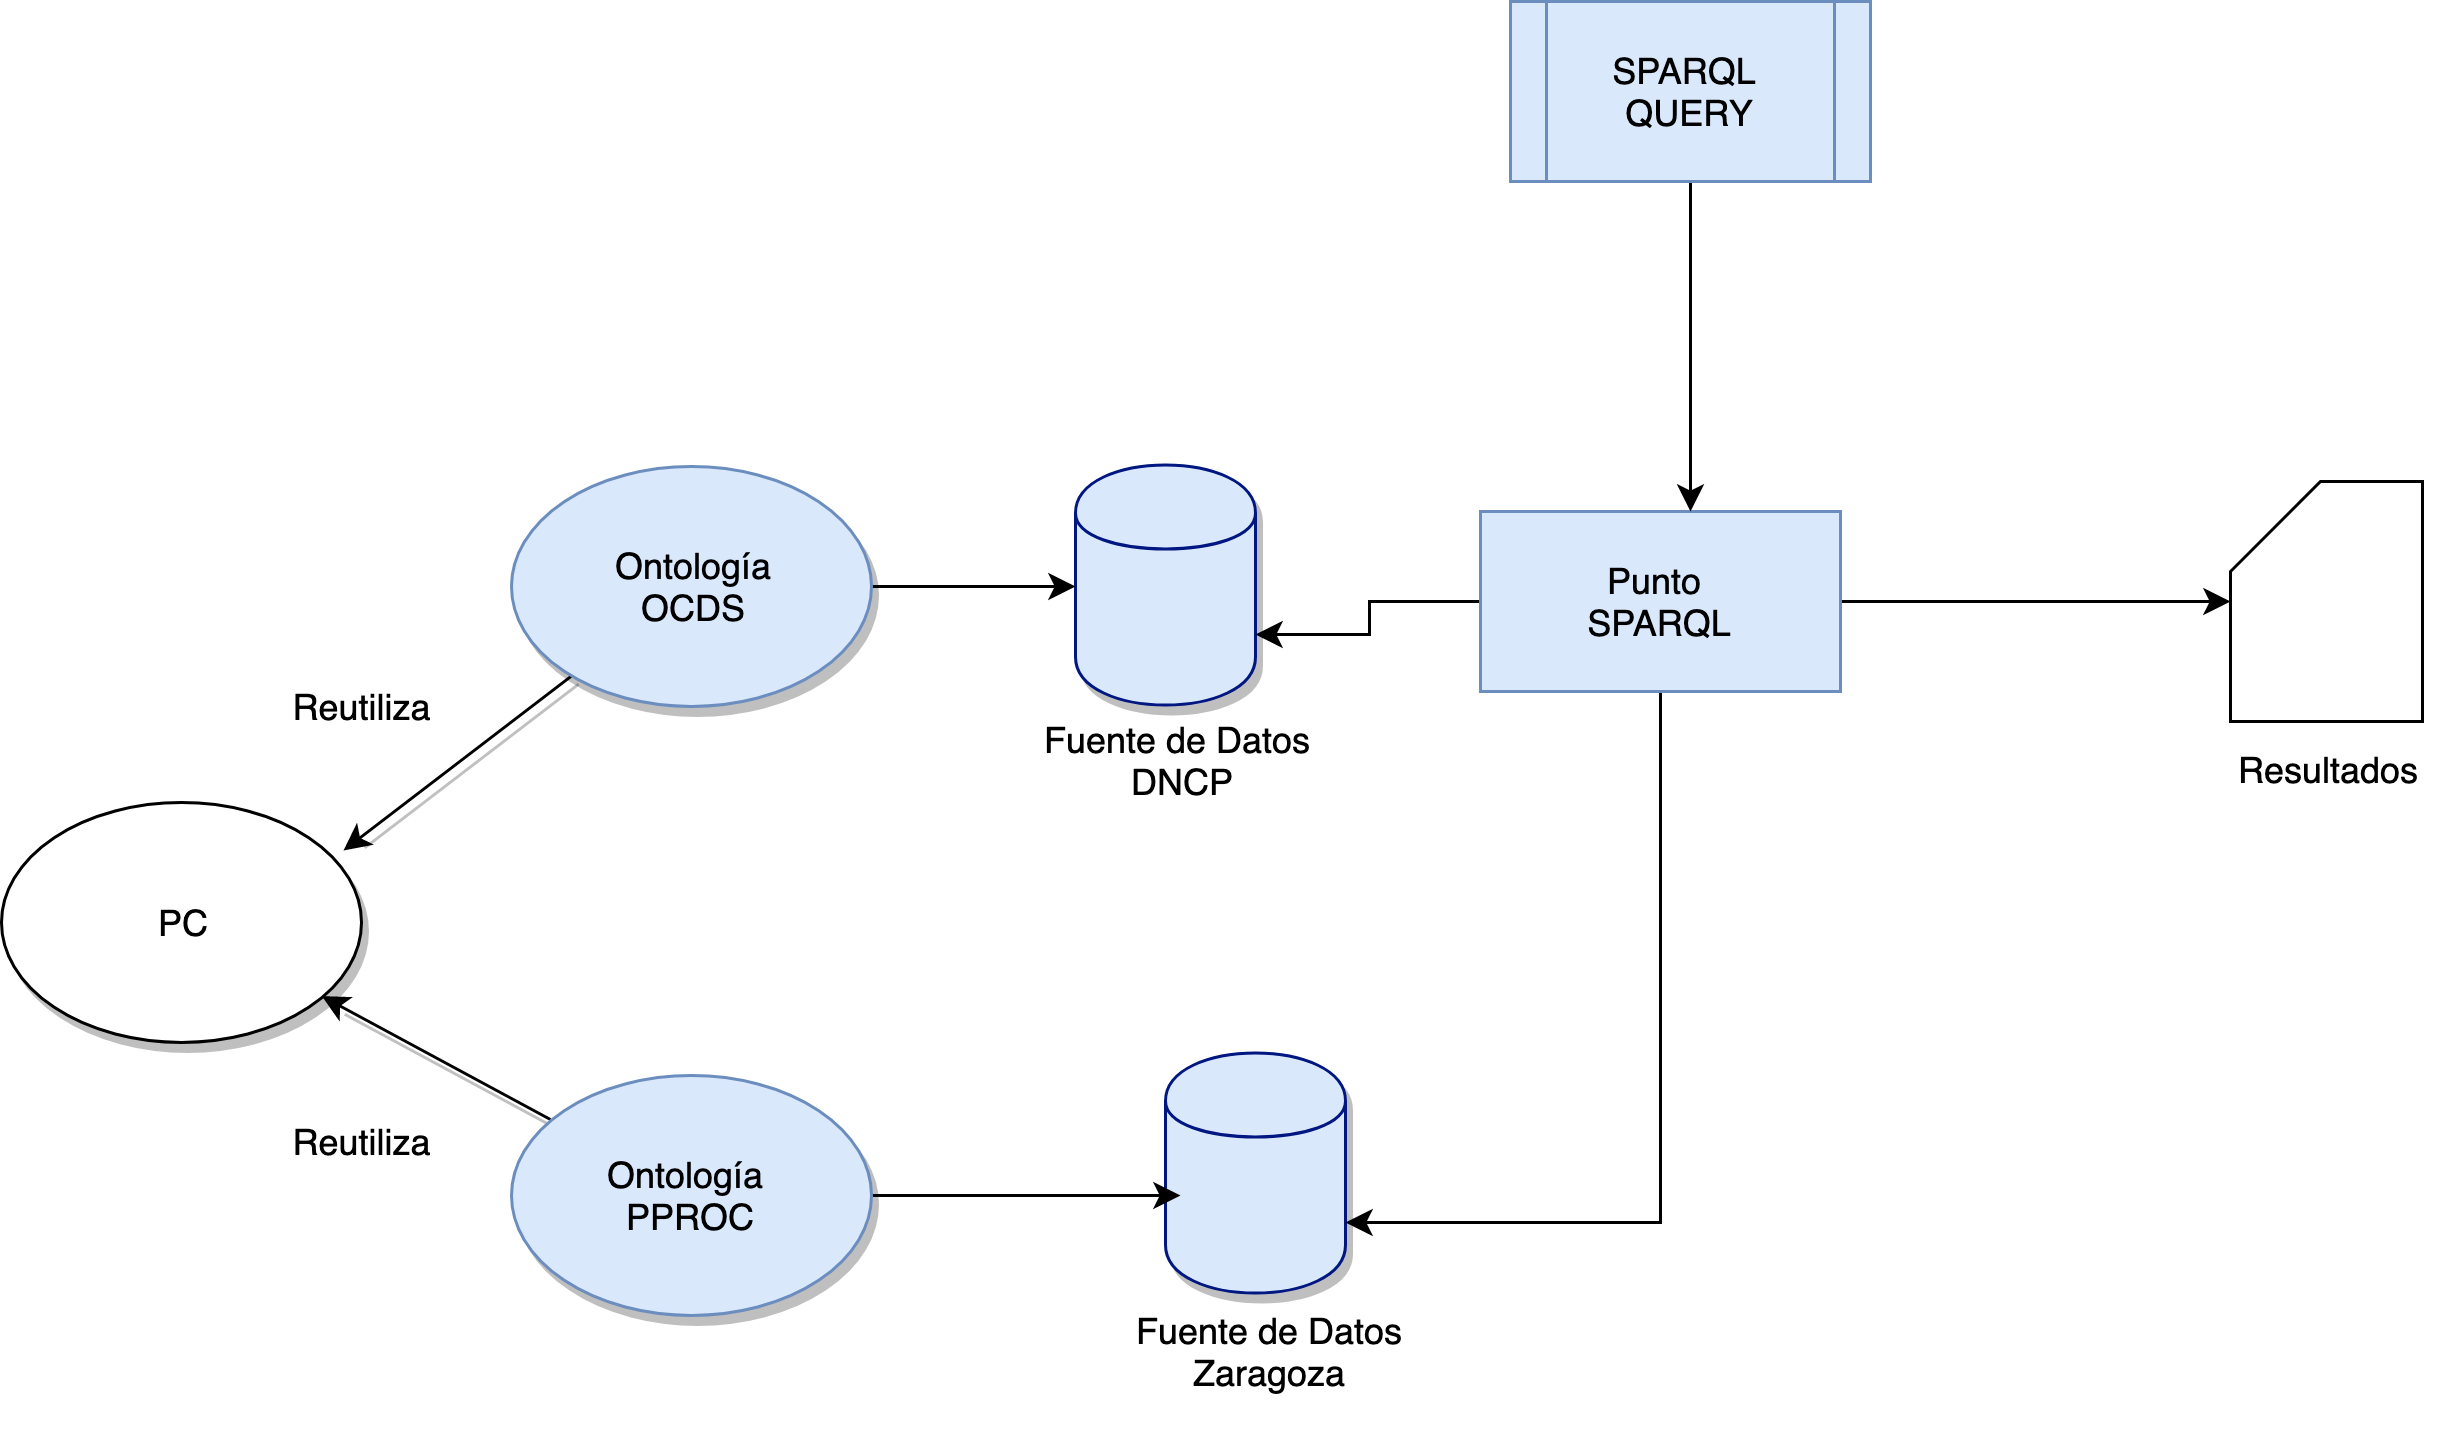
\includegraphics[width=150mm]{figuras/Diagramas-Caso4.png}
    \caption{Diagrama de la consulta del caso 4}
    \label{img:Diagramas-Caso 4}
 \end{figure}
